\begin{savequote}[75mm] 
Quality is never an accident; it is always the result of intelligent effort. 
\qauthor{John Ruskin.} 
\end{savequote}


\chapter{UT test beam analysis - a measurement of the charge sharing
in planar silicon sensors}
\label{chapter:testbeam}

This chapter is dedicated to describes the testbeam studies performed on prototypes of silicon microstrip sensors that will build the Upstream Tracker.  The chapter starts by presenting the general idea of the testbeam experiments, followed by a section on an experimental setup. The final section describes the study on charge sharing phenomena and the proposed correction. 

\section{Experimental setup}

\subsection{The beam}
The tests were performed in CERN SPS North Area see figure \ref{fig:LHC}. The beam consisted of secondary particles produced by the interaction of high intensity of 450 GeV/c primary proton beam with a fixed target made of beryllium and lead. The beam had average energy of $180 GeV$.  
The beam typically produced four spills/minute. The spill lasted about 4 seconds, and it was intermittent by 40 seconds window with no beam. For most of the data taking, the beam size was collimated down to about 0.5 cm in diameter.

\subsection{Timepix3 telescope}
The essential tool that allows making many silicon sensor performance studies is the TimePix3 telescope, presented in figure \ref{fig:telescope}. 


\begin{figure}[!h]
\centering
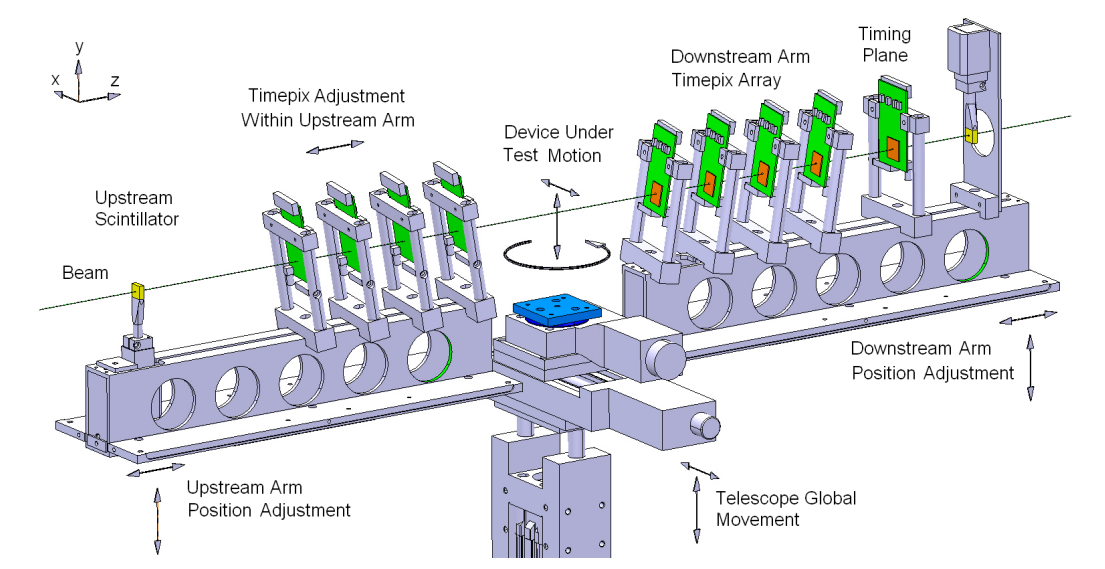
\includegraphics{figures/telescope.png}
\caption{Layout of the Timepix Telescope mechanics, pixel planes and scintillators with respect to the beam axis. Figure taken from \cite{telescope}}
\label{fig:telescope}
\end{figure}


This device consists of 8 plates of 300 $\mum$ thick p-on-n sensors bump bonded to the Timepix3 ASIC, divided equally between two arms. The position of each plate along the z-axis is adjustable, typically the distance between each plate is set to be 31 mm, and plates are rotated to an angle of 9 deg in both x and y-axis to improve position reconstruction. There is a 200 mm gap between two telescope arms, which is used to place Device Under Test (DUT), see photo \ref{fig:telescope_photo} taken during one of the testbeam companies. The DUT is housed inside a metal box designed to fit into the gap and provides an airtight dry environment cooled via a Peltier device. 
The DUT was installed on a motion stage allowing angular rotations and x and y translations. 

To allow the DUT acquisition to trigger two scintillators are placed upstream and downstream of the telescope. The telescope acquisition system does not require any trigger signal since it works in a so-called data-driven read-out mode in which the data package of each pixel hit is sent immediately after Time-over-Threshold (ToT) conversion. To synchronize DUT clusters with associated Telescope tracks, the information about the trigger timestamp is added to the data recorded by the telescope.  


\begin{figure}[!h]
\centering
\hspace*{-1cm}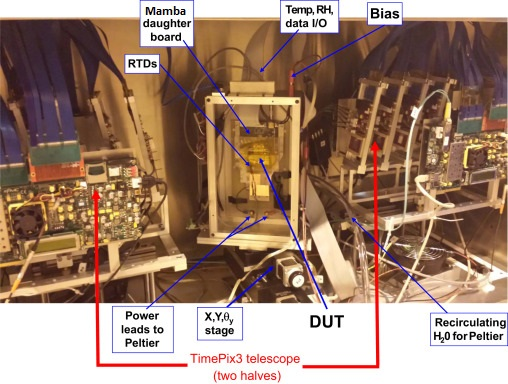
\includegraphics{figures/telescope_photo.jpg}
\caption{The photo of the Timepix Telescope and the DUT inside the box. }
\label{fig:telescope_photo}
\end{figure}

\subsubsection{TimePix3 Telescope Tracking}

To find the position where the particle interacts with the DUT sensor, the particle trajectory needs to be reconstructed using the information provided by all Telescope plates. This procedure starts by finding clusters. The cluster is a collection of neighboring pixels in which the measured signal exceeds a certain threshold, and such a measurement is called a hit. The hit is created when a charged particle traverses through the sensor.  To add the hit to the cluster, its timestamp must lie within the 100 nanosecond window surrounding the timestamp of the seed hit. The timestamp of the cluster is a minimum of the timestamps associated with each of the hits belonging to the cluster. The cluster charge is a sum of charges of the constituent hits. 
The x and y positions of the cluster are calculated using the center of gravity method: 

\begin{equation}
    \{x,y\}_{cluster} = \frac{\sum_{i = 0}^{n} \{x,y\}_{i} S_{i}}{\sum_{i = 0}^{n} S_{i}} 
\end{equation}
where $\{x,y\}_{i} $ is the $x$ or $y$  coordinates of $i$th pixel and $S_i$ its signal. 

The clusters are then used as input for the tracking algorithm, which is based on the timing information of the clusters.  The tracking algorithm starts by taking a cluster form the first plane and then looks for the matching cluster on the second plane. The hits are considered matched when the time difference is within ten nanoseconds. These two clusters constitute a track seed which is then extrapolated to the next plane, excluding the device under test, looking for a cluster within a cone with an opening angle of 0.01 radians and the ten ns time window. The procedure ends when all planes have been considered. Figure \ref{fig:telescope_tracks} shows four examples of Timepix3 tracks. 



\begin{figure}
\centering
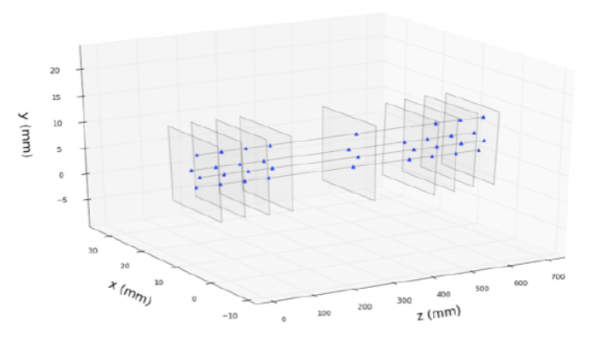
\includegraphics[scale=0.9]{figures/telescope_tracks.png}
\caption{Four example tracks reconstructed in the Timepix3 telescope. Figure taken from \cite{Sophie}.}
\label{fig:telescope_tracks}
\end{figure}


\subsection{Read-out electronic}
During all of the testbeam experiments conducted from 2015 till 2017, the SALT ASIC was not ready. Therefore, the sensor was read-out by the Beetle chip, which is the ASIC used as a front-end chip in Velo and TT. The Beetle chip can read-out the signals from 128 channels and returns semi-Gaussian analog pules.  The detailed description of the Beetle chip data processing can be found \cite{Beetle}.  In contrary to the SALT ASIC, the Beetle chip has no digital signal processing module. Thus, data have to digitalized and processed by the external components.  
The analog data read-out by the Beetle chip was digitalized by the Mamba board designed by INFN in Milan and produced by Nuclear Instrument \cite{}.   
The processing of the digitalized data was done by the software described in chapter \ref{chapter:tbut}. 

\section{Testbeam studies and the results}
The 

\section{Charge sharing}
This section focuses on the analysis of charge sharing. Charge sharing occurs when a particle deposits charge between two strips, see figure \ref{fig:charge_Sharing}. The precision at which the position of a charged particle can be reconstructed is dependent on how charge is shared between
In this case, the charge can flow to both the left and right strips.  
This phenomenon can be quantified via parameter $\eta$ given by:

\begin{equation}
    \eta = \frac{Q_{left}}{Q_{left}+Q_{right}}
\end{equation}


\section{Charge sharing correction}
